\begin{figure}[t]
	\begin{center}








\tikzset{every picture/.style={line width=0.75pt}} %set default line width to 0.75pt        

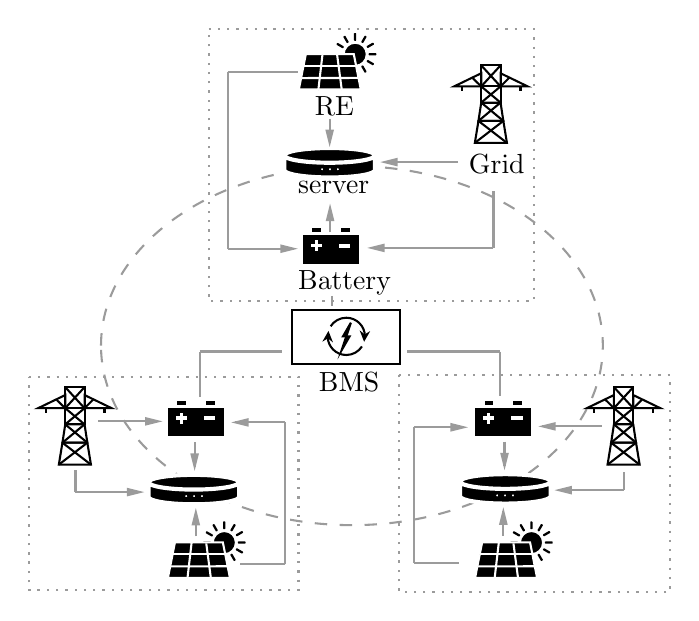
\begin{tikzpicture}[x=0.75pt,y=0.75pt,yscale=-1,xscale=1]
%uncomment if require: \path (0,446); %set diagram left start at 0, and has height of 446

%Shape: Ellipse [id:dp0609926737364892] 
\draw  [color={rgb, 255:red, 155; green, 155; blue, 155 }  ,draw opacity=1 ][dash pattern={on 4.5pt off 4.5pt}] (38.5,155.68) .. controls (38.5,107.91) and (92.62,69.18) .. (159.39,69.18) .. controls (226.15,69.18) and (280.28,107.91) .. (280.28,155.68) .. controls (280.28,203.45) and (226.15,242.18) .. (159.39,242.18) .. controls (92.62,242.18) and (38.5,203.45) .. (38.5,155.68) -- cycle ;
%Shape: Ellipse [id:dp23689960204771032] 
\draw  [color={rgb, 255:red, 255; green, 255; blue, 255 }  ,draw opacity=1 ][fill={rgb, 255:red, 0; green, 0; blue, 0 }  ,fill opacity=1 ] (155.38,15.32) .. controls (155.38,12.23) and (157.89,9.73) .. (160.97,9.73) .. controls (164.06,9.73) and (166.56,12.23) .. (166.56,15.32) .. controls (166.56,18.41) and (164.06,20.91) .. (160.97,20.91) .. controls (157.89,20.91) and (155.38,18.41) .. (155.38,15.32) -- cycle ;
%Rounded Rect [id:dp7350954357882564] 
\draw   (167.98,15.27) .. controls (167.98,15.26) and (167.99,15.25) .. (168,15.25) -- (170.69,15.25) .. controls (170.7,15.25) and (170.71,15.26) .. (170.71,15.27) -- (170.71,15.32) .. controls (170.71,15.33) and (170.7,15.34) .. (170.69,15.34) -- (168,15.34) .. controls (167.99,15.34) and (167.98,15.33) .. (167.98,15.32) -- cycle ;
%Rounded Rect [id:dp5817858075714595] 
\draw   (152.56,10.42) .. controls (152.57,10.41) and (152.58,10.4) .. (152.59,10.41) -- (154.92,11.76) .. controls (154.93,11.76) and (154.93,11.77) .. (154.93,11.78) -- (154.9,11.83) .. controls (154.89,11.84) and (154.88,11.84) .. (154.87,11.84) -- (152.54,10.49) .. controls (152.53,10.48) and (152.53,10.47) .. (152.53,10.46) -- cycle ;
%Rounded Rect [id:dp562001902201841] 
\draw   (155.9,6.97) .. controls (155.91,6.96) and (155.92,6.96) .. (155.92,6.97) -- (157.27,9.31) .. controls (157.27,9.31) and (157.27,9.32) .. (157.26,9.33) -- (157.22,9.36) .. controls (157.21,9.36) and (157.2,9.36) .. (157.19,9.35) -- (155.84,7.02) .. controls (155.84,7.01) and (155.84,7) .. (155.85,6.99) -- cycle ;
%Rounded Rect [id:dp24994446560754513] 
\draw   (160.96,5.61) .. controls (160.97,5.61) and (160.97,5.61) .. (160.97,5.62) -- (160.97,8.32) .. controls (160.97,8.33) and (160.97,8.34) .. (160.96,8.34) -- (160.9,8.34) .. controls (160.89,8.34) and (160.88,8.33) .. (160.88,8.32) -- (160.88,5.62) .. controls (160.88,5.61) and (160.89,5.61) .. (160.9,5.61) -- cycle ;
%Rounded Rect [id:dp41080675695046875] 
\draw   (151.26,15.25) .. controls (151.26,15.24) and (151.27,15.23) .. (151.28,15.23) -- (153.97,15.23) .. controls (153.98,15.23) and (153.99,15.24) .. (153.99,15.25) -- (153.99,15.3) .. controls (153.99,15.31) and (153.98,15.32) .. (153.97,15.32) -- (151.28,15.32) .. controls (151.27,15.32) and (151.26,15.31) .. (151.26,15.3) -- cycle ;
%Rounded Rect [id:dp2589224672963768] 
\draw   (164.51,21.23) .. controls (164.52,21.23) and (164.53,21.23) .. (164.54,21.24) -- (165.88,23.57) .. controls (165.89,23.58) and (165.89,23.59) .. (165.88,23.6) -- (165.83,23.62) .. controls (165.82,23.63) and (165.81,23.63) .. (165.8,23.62) -- (164.46,21.28) .. controls (164.45,21.28) and (164.46,21.26) .. (164.46,21.26) -- cycle ;
%Rounded Rect [id:dp52965196080424] 
\draw   (161.05,22.31) .. controls (161.06,22.31) and (161.06,22.32) .. (161.06,22.33) -- (161.06,25.02) .. controls (161.06,25.03) and (161.06,25.04) .. (161.05,25.04) -- (160.99,25.04) .. controls (160.98,25.04) and (160.97,25.03) .. (160.97,25.02) -- (160.97,22.33) .. controls (160.97,22.32) and (160.98,22.31) .. (160.99,22.31) -- cycle ;
%Rounded Rect [id:dp4402538190695453] 
\draw   (167.1,18.63) .. controls (167.1,18.62) and (167.11,18.61) .. (167.12,18.62) -- (169.46,19.97) .. controls (169.46,19.97) and (169.47,19.98) .. (169.46,19.99) -- (169.43,20.04) .. controls (169.43,20.05) and (169.42,20.05) .. (169.41,20.05) -- (167.08,18.7) .. controls (167.07,18.69) and (167.07,18.68) .. (167.07,18.67) -- cycle ;
%Rounded Rect [id:dp6996007283347523] 
\draw   (165.88,6.96) .. controls (165.89,6.96) and (165.89,6.97) .. (165.88,6.98) -- (164.54,9.31) .. controls (164.53,9.32) and (164.52,9.33) .. (164.51,9.32) -- (164.46,9.29) .. controls (164.46,9.29) and (164.45,9.28) .. (164.46,9.27) -- (165.8,6.94) .. controls (165.81,6.93) and (165.82,6.92) .. (165.83,6.93) -- cycle ;
%Rounded Rect [id:dp670060683107357] 
\draw   (169.46,10.34) .. controls (169.47,10.35) and (169.46,10.36) .. (169.46,10.37) -- (167.12,11.71) .. controls (167.11,11.72) and (167.1,11.72) .. (167.1,11.71) -- (167.07,11.66) .. controls (167.07,11.65) and (167.07,11.64) .. (167.08,11.63) -- (169.41,10.29) .. controls (169.42,10.28) and (169.43,10.29) .. (169.43,10.29) -- cycle ;
%Rounded Rect [id:dp17906894780647287] 
\draw   (154.93,18.55) .. controls (154.93,18.56) and (154.93,18.57) .. (154.92,18.58) -- (152.59,19.92) .. controls (152.58,19.93) and (152.57,19.93) .. (152.56,19.92) -- (152.53,19.87) .. controls (152.53,19.86) and (152.53,19.85) .. (152.54,19.84) -- (154.87,18.5) .. controls (154.88,18.49) and (154.89,18.5) .. (154.9,18.5) -- cycle ;
%Rounded Rect [id:dp7163585653714504] 
\draw   (157.13,21.22) .. controls (157.14,21.23) and (157.14,21.24) .. (157.13,21.25) -- (155.79,23.58) .. controls (155.78,23.59) and (155.77,23.59) .. (155.76,23.59) -- (155.72,23.56) .. controls (155.71,23.55) and (155.7,23.54) .. (155.71,23.54) -- (157.06,21.2) .. controls (157.06,21.19) and (157.07,21.19) .. (157.08,21.2) -- cycle ;

%Shape: Trapezoid [id:dp39839281755362443] 
\draw  [color={rgb, 255:red, 255; green, 255; blue, 255 }  ,draw opacity=1 ][fill={rgb, 255:red, 0; green, 0; blue, 0 }  ,fill opacity=1 ] (133.8,32.28) -- (137.2,15.21) -- (160.28,15.21) -- (163.68,32.28) -- cycle ;
%Straight Lines [id:da8047810174415737] 
\draw [color={rgb, 255:red, 255; green, 255; blue, 255 }  ,draw opacity=1 ][fill={rgb, 255:red, 0; green, 0; blue, 0 }  ,fill opacity=1 ]   (135.05,26.77) -- (162.64,26.72) ;
%Straight Lines [id:da8343675725090776] 
\draw [color={rgb, 255:red, 255; green, 255; blue, 255 }  ,draw opacity=1 ][fill={rgb, 255:red, 0; green, 0; blue, 0 }  ,fill opacity=1 ]   (136,20.82) -- (161.09,20.82) ;
%Straight Lines [id:da6746426481591967] 
\draw [color={rgb, 255:red, 255; green, 255; blue, 255 }  ,draw opacity=1 ][fill={rgb, 255:red, 0; green, 0; blue, 0 }  ,fill opacity=1 ]   (152.28,15.7) -- (154.51,32.54) ;
%Straight Lines [id:da546227329864996] 
\draw [color={rgb, 255:red, 255; green, 255; blue, 255 }  ,draw opacity=1 ][fill={rgb, 255:red, 0; green, 0; blue, 0 }  ,fill opacity=1 ]   (145.19,15.54) -- (143.19,32.66) ;


%Shape: Can [id:dp9005011599408153] 
\draw  [color={rgb, 255:red, 255; green, 255; blue, 255 }  ,draw opacity=1 ][fill={rgb, 255:red, 0; green, 0; blue, 0 }  ,fill opacity=1 ][line width=1.5]  (170.53,64.02) -- (170.53,71.12) .. controls (170.53,73.08) and (160.74,74.67) .. (148.67,74.67) .. controls (136.6,74.67) and (126.82,73.08) .. (126.82,71.12) -- (126.82,64.02) .. controls (126.82,62.06) and (136.6,60.47) .. (148.67,60.47) .. controls (160.74,60.47) and (170.53,62.06) .. (170.53,64.02) .. controls (170.53,65.98) and (160.74,67.57) .. (148.67,67.57) .. controls (136.6,67.57) and (126.82,65.98) .. (126.82,64.02) ;
%Shape: Ellipse [id:dp627980002725933] 
\draw  [fill={rgb, 255:red, 255; green, 255; blue, 255 }  ,fill opacity=1 ] (147.75,70.72) .. controls (147.75,70.13) and (148.23,69.65) .. (148.82,69.65) .. controls (149.41,69.65) and (149.89,70.13) .. (149.89,70.72) .. controls (149.89,71.31) and (149.41,71.79) .. (148.82,71.79) .. controls (148.23,71.79) and (147.75,71.31) .. (147.75,70.72) -- cycle ;
%Shape: Ellipse [id:dp32022930297328456] 
\draw  [fill={rgb, 255:red, 255; green, 255; blue, 255 }  ,fill opacity=1 ] (151.55,70.72) .. controls (151.55,70.13) and (152.02,69.65) .. (152.62,69.65) .. controls (153.21,69.65) and (153.68,70.13) .. (153.68,70.72) .. controls (153.68,71.31) and (153.21,71.79) .. (152.62,71.79) .. controls (152.02,71.79) and (151.55,71.31) .. (151.55,70.72) -- cycle ;
%Shape: Ellipse [id:dp09464548947851847] 
\draw  [fill={rgb, 255:red, 255; green, 255; blue, 255 }  ,fill opacity=1 ] (143.96,70.72) .. controls (143.96,70.13) and (144.44,69.65) .. (145.03,69.65) .. controls (145.62,69.65) and (146.1,70.13) .. (146.1,70.72) .. controls (146.1,71.31) and (145.62,71.79) .. (145.03,71.79) .. controls (144.44,71.79) and (143.96,71.31) .. (143.96,70.72) -- cycle ;

%Shape: Rectangle [id:dp35865913094459034] 
\draw  [fill={rgb, 255:red, 0; green, 0; blue, 0 }  ,fill opacity=1 ] (136.18,102.97) -- (162.32,102.97) -- (162.32,115.73) -- (136.18,115.73) -- cycle ;
%Shape: Cross [id:dp9459558747780203] 
\draw  [fill={rgb, 255:red, 255; green, 255; blue, 255 }  ,fill opacity=1 ] (143.64,104.38) -- (140.99,104.38) -- (140.99,106.25) -- (139.12,106.25) -- (139.12,108.9) -- (140.99,108.9) -- (140.99,110.76) -- (143.64,110.76) -- (143.64,108.9) -- (145.51,108.9) -- (145.51,106.25) -- (143.64,106.25) -- cycle ;
%Shape: Rectangle [id:dp8159450856522705] 
\draw  [fill={rgb, 255:red, 255; green, 255; blue, 255 }  ,fill opacity=1 ] (152.74,106.11) -- (159.17,106.11) -- (159.17,108.98) -- (152.74,108.98) -- cycle ;
%Shape: Rectangle [id:dp9559476182094357] 
\draw  [fill={rgb, 255:red, 0; green, 0; blue, 0 }  ,fill opacity=1 ] (140.83,99.67) -- (144.1,99.67) -- (144.1,100.66) -- (140.83,100.66) -- cycle ;
%Shape: Rectangle [id:dp06489231659707517] 
\draw  [fill={rgb, 255:red, 0; green, 0; blue, 0 }  ,fill opacity=1 ] (154.7,99.67) -- (157.96,99.67) -- (157.96,100.66) -- (154.7,100.66) -- cycle ;

%Shape: Trapezoid [id:dp5856244719833053] 
\draw   (218.62,58) -- (220.35,47.43) -- (232.35,47.43) -- (234.08,58) -- cycle ;
%Shape: Trapezoid [id:dp44335621565613703] 
\draw   (220.35,47.43) -- (221.7,38.59) -- (231,38.59) -- (232.35,47.43) -- cycle ;
%Shape: Trapezoid [id:dp2690273077646286] 
\draw   (221.7,38.59) -- (221.7,30.8) -- (231,30.8) -- (231,38.59) -- cycle ;
%Shape: Trapezoid [id:dp789123773409603] 
\draw   (221.7,30.8) -- (221.7,20.67) -- (231,20.67) -- (231,30.8) -- cycle ;
%Straight Lines [id:da828316850046003] 
\draw    (220.35,47.43) -- (234.08,58) ;
%Straight Lines [id:da591569368482918] 
\draw    (218.62,58) -- (232.35,47.43) ;
%Straight Lines [id:da7192792870901867] 
\draw    (220.35,47.43) -- (231,38.59) ;
%Straight Lines [id:da25942426045741995] 
\draw    (232.35,47.43) -- (221.7,38.59) ;
%Straight Lines [id:da998802426261975] 
\draw    (231,38.59) -- (221.7,30.8) ;
%Straight Lines [id:da38916705477465796] 
\draw    (221.7,38.59) -- (231,30.8) ;
%Straight Lines [id:da26657305293991884] 
\draw    (221.7,30.8) -- (231,20.67) ;
%Straight Lines [id:da31720929903327444] 
\draw    (231,30.8) -- (221.7,20.67) ;
%Shape: Right Triangle [id:dp46306371951470315] 
\draw   (231,24.47) -- (244.07,30.8) -- (231,30.8) -- cycle ;
%Straight Lines [id:da5846990799110421] 
\draw    (231,30.8) -- (235.28,26.53) ;
%Straight Lines [id:da9958530803374206] 
\draw    (240.62,30.93) -- (240.62,33.07) ;

%Shape: Right Triangle [id:dp09576900324503912] 
\draw   (221.7,24.47) -- (208.63,30.8) -- (221.7,30.8) -- cycle ;
%Straight Lines [id:da10297154407621023] 
\draw    (217.55,26.8) -- (221.7,30.8) ;
%Straight Lines [id:da9008160700393986] 
\draw    (212.22,30.93) -- (212.22,33.07) ;

%Straight Lines [id:da061465447579204024] 
\draw [color={rgb, 255:red, 155; green, 155; blue, 155 }  ,draw opacity=1 ]   (227.6,108.6) -- (227.6,81) ;
%Straight Lines [id:da29204250583497604] 
\draw [color={rgb, 255:red, 155; green, 155; blue, 155 }  ,draw opacity=1 ]   (99.47,23.7) -- (133.3,23.7) ;
%Straight Lines [id:da7117577732035187] 
\draw [color={rgb, 255:red, 155; green, 155; blue, 155 }  ,draw opacity=1 ]   (99.47,23.7) -- (99.47,109) ;
%Straight Lines [id:da03215825036288611] 
\draw [color={rgb, 255:red, 155; green, 155; blue, 155 }  ,draw opacity=1 ]   (99.47,109) -- (131.3,109) ;
\draw [shift={(133.3,109)}, rotate = 180] [fill={rgb, 255:red, 155; green, 155; blue, 155 }  ,fill opacity=1 ][line width=0.08]  [draw opacity=0] (8.4,-2.1) -- (0,0) -- (8.4,2.1) -- cycle    ;
%Straight Lines [id:da15100116685442955] 
\draw [color={rgb, 255:red, 155; green, 155; blue, 155 }  ,draw opacity=1 ]   (148.86,100.97) -- (148.86,89.26) ;
\draw [shift={(148.86,87.26)}, rotate = 90] [fill={rgb, 255:red, 155; green, 155; blue, 155 }  ,fill opacity=1 ][line width=0.08]  [draw opacity=0] (8.4,-2.1) -- (0,0) -- (8.4,2.1) -- cycle    ;
%Straight Lines [id:da9367614692819763] 
\draw [color={rgb, 255:red, 155; green, 155; blue, 155 }  ,draw opacity=1 ]   (148.67,46.26) -- (148.67,57.97) ;
\draw [shift={(148.67,59.97)}, rotate = 270] [fill={rgb, 255:red, 155; green, 155; blue, 155 }  ,fill opacity=1 ][line width=0.08]  [draw opacity=0] (8.4,-2.1) -- (0,0) -- (8.4,2.1) -- cycle    ;
%Straight Lines [id:da8205726453259106] 
\draw [color={rgb, 255:red, 155; green, 155; blue, 155 }  ,draw opacity=1 ]   (210.5,67.26) -- (175.07,67.26) ;
\draw [shift={(173.07,67.26)}, rotate = 360] [fill={rgb, 255:red, 155; green, 155; blue, 155 }  ,fill opacity=1 ][line width=0.08]  [draw opacity=0] (8.4,-2.1) -- (0,0) -- (8.4,2.1) -- cycle    ;
%Straight Lines [id:da9417145681951029] 
\draw [color={rgb, 255:red, 155; green, 155; blue, 155 }  ,draw opacity=1 ]   (227.6,108.6) -- (168.8,108.6) ;
\draw [shift={(166.8,108.6)}, rotate = 360] [fill={rgb, 255:red, 155; green, 155; blue, 155 }  ,fill opacity=1 ][line width=0.08]  [draw opacity=0] (8.4,-2.1) -- (0,0) -- (8.4,2.1) -- cycle    ;
%Shape: Ellipse [id:dp046440233113860696] 
\draw  [color={rgb, 255:red, 255; green, 255; blue, 255 }  ,draw opacity=1 ][fill={rgb, 255:red, 0; green, 0; blue, 0 }  ,fill opacity=1 ] (92.32,250.59) .. controls (92.32,247.5) and (94.82,245) .. (97.91,245) .. controls (100.99,245) and (103.5,247.5) .. (103.5,250.59) .. controls (103.5,253.68) and (100.99,256.18) .. (97.91,256.18) .. controls (94.82,256.18) and (92.32,253.68) .. (92.32,250.59) -- cycle ;
%Rounded Rect [id:dp21673028923709814] 
\draw   (104.91,250.53) .. controls (104.91,250.52) and (104.92,250.52) .. (104.93,250.52) -- (107.62,250.52) .. controls (107.63,250.52) and (107.64,250.52) .. (107.64,250.53) -- (107.64,250.59) .. controls (107.64,250.6) and (107.63,250.61) .. (107.62,250.61) -- (104.93,250.61) .. controls (104.92,250.61) and (104.91,250.6) .. (104.91,250.59) -- cycle ;
%Rounded Rect [id:dp9417842391430391] 
\draw   (89.5,245.68) .. controls (89.5,245.67) and (89.51,245.67) .. (89.52,245.68) -- (91.85,247.02) .. controls (91.86,247.03) and (91.86,247.04) .. (91.86,247.05) -- (91.83,247.1) .. controls (91.83,247.1) and (91.82,247.11) .. (91.81,247.1) -- (89.47,245.75) .. controls (89.47,245.75) and (89.46,245.74) .. (89.47,245.73) -- cycle ;
%Rounded Rect [id:dp4967499642080284] 
\draw   (92.83,242.23) .. controls (92.84,242.23) and (92.85,242.23) .. (92.86,242.24) -- (94.2,244.57) .. controls (94.21,244.58) and (94.2,244.59) .. (94.2,244.6) -- (94.15,244.62) .. controls (94.14,244.63) and (94.13,244.63) .. (94.12,244.62) -- (92.78,242.28) .. controls (92.77,242.28) and (92.78,242.26) .. (92.78,242.26) -- cycle ;
%Rounded Rect [id:dp42182766171645003] 
\draw   (97.89,240.87) .. controls (97.9,240.87) and (97.91,240.88) .. (97.91,240.89) -- (97.91,243.58) .. controls (97.91,243.59) and (97.9,243.6) .. (97.89,243.6) -- (97.83,243.6) .. controls (97.82,243.6) and (97.82,243.59) .. (97.82,243.58) -- (97.82,240.89) .. controls (97.82,240.88) and (97.82,240.87) .. (97.83,240.87) -- cycle ;
%Rounded Rect [id:dp7372953483874027] 
\draw   (88.19,250.52) .. controls (88.19,250.51) and (88.2,250.5) .. (88.21,250.5) -- (90.9,250.5) .. controls (90.91,250.5) and (90.92,250.51) .. (90.92,250.52) -- (90.92,250.57) .. controls (90.92,250.58) and (90.91,250.59) .. (90.9,250.59) -- (88.21,250.59) .. controls (88.2,250.59) and (88.19,250.58) .. (88.19,250.57) -- cycle ;
%Rounded Rect [id:dp016554811734768915] 
\draw   (101.44,256.5) .. controls (101.45,256.49) and (101.46,256.5) .. (101.47,256.51) -- (102.82,258.84) .. controls (102.82,258.85) and (102.82,258.86) .. (102.81,258.86) -- (102.76,258.89) .. controls (102.75,258.9) and (102.74,258.89) .. (102.74,258.88) -- (101.39,256.55) .. controls (101.39,256.54) and (101.39,256.53) .. (101.4,256.53) -- cycle ;
%Rounded Rect [id:dp3333806907098691] 
\draw   (97.98,257.57) .. controls (97.99,257.57) and (98,257.58) .. (98,257.59) -- (98,260.29) .. controls (98,260.3) and (97.99,260.3) .. (97.98,260.3) -- (97.92,260.3) .. controls (97.91,260.3) and (97.91,260.3) .. (97.91,260.29) -- (97.91,257.59) .. controls (97.91,257.58) and (97.91,257.57) .. (97.92,257.57) -- cycle ;
%Rounded Rect [id:dp4045437830291596] 
\draw   (104.03,253.89) .. controls (104.04,253.88) and (104.05,253.88) .. (104.06,253.89) -- (106.39,255.23) .. controls (106.4,255.24) and (106.4,255.25) .. (106.4,255.26) -- (106.37,255.31) .. controls (106.36,255.31) and (106.35,255.32) .. (106.34,255.31) -- (104.01,253.96) .. controls (104,253.96) and (104,253.95) .. (104,253.94) -- cycle ;
%Rounded Rect [id:dp18140925314320766] 
\draw   (102.81,242.22) .. controls (102.82,242.23) and (102.82,242.24) .. (102.82,242.25) -- (101.47,244.58) .. controls (101.46,244.59) and (101.45,244.59) .. (101.44,244.59) -- (101.4,244.56) .. controls (101.39,244.56) and (101.39,244.54) .. (101.39,244.54) -- (102.74,242.2) .. controls (102.74,242.19) and (102.75,242.19) .. (102.76,242.2) -- cycle ;
%Rounded Rect [id:dp6960166673215535] 
\draw   (106.4,245.61) .. controls (106.4,245.62) and (106.4,245.63) .. (106.39,245.63) -- (104.06,246.98) .. controls (104.05,246.98) and (104.04,246.98) .. (104.03,246.97) -- (104,246.93) .. controls (104,246.92) and (104,246.91) .. (104.01,246.9) -- (106.34,245.55) .. controls (106.35,245.55) and (106.36,245.55) .. (106.37,245.56) -- cycle ;
%Rounded Rect [id:dp34185776666936607] 
\draw   (91.86,253.82) .. controls (91.86,253.83) and (91.86,253.84) .. (91.85,253.84) -- (89.52,255.19) .. controls (89.51,255.19) and (89.5,255.19) .. (89.5,255.18) -- (89.47,255.14) .. controls (89.46,255.13) and (89.47,255.12) .. (89.47,255.11) -- (91.81,253.76) .. controls (91.82,253.76) and (91.83,253.76) .. (91.83,253.77) -- cycle ;
%Rounded Rect [id:dp5556414628284645] 
\draw   (94.06,256.49) .. controls (94.07,256.49) and (94.07,256.51) .. (94.07,256.51) -- (92.72,258.85) .. controls (92.72,258.86) and (92.71,258.86) .. (92.7,258.85) -- (92.65,258.83) .. controls (92.64,258.82) and (92.64,258.81) .. (92.64,258.8) -- (93.99,256.47) .. controls (93.99,256.46) and (94.01,256.46) .. (94.01,256.46) -- cycle ;

%Shape: Trapezoid [id:dp9078658261484358] 
\draw  [color={rgb, 255:red, 255; green, 255; blue, 255 }  ,draw opacity=1 ][fill={rgb, 255:red, 0; green, 0; blue, 0 }  ,fill opacity=1 ] (70.73,267.55) -- (74.13,250.48) -- (97.21,250.48) -- (100.61,267.55) -- cycle ;
%Straight Lines [id:da6538397825350515] 
\draw [color={rgb, 255:red, 255; green, 255; blue, 255 }  ,draw opacity=1 ][fill={rgb, 255:red, 0; green, 0; blue, 0 }  ,fill opacity=1 ]   (71.98,262.04) -- (99.58,261.99) ;
%Straight Lines [id:da5435454566868603] 
\draw [color={rgb, 255:red, 255; green, 255; blue, 255 }  ,draw opacity=1 ][fill={rgb, 255:red, 0; green, 0; blue, 0 }  ,fill opacity=1 ]   (72.94,256.09) -- (98.02,256.09) ;
%Straight Lines [id:da24497164177888142] 
\draw [color={rgb, 255:red, 255; green, 255; blue, 255 }  ,draw opacity=1 ][fill={rgb, 255:red, 0; green, 0; blue, 0 }  ,fill opacity=1 ]   (89.21,250.97) -- (91.45,267.81) ;
%Straight Lines [id:da32161055867429855] 
\draw [color={rgb, 255:red, 255; green, 255; blue, 255 }  ,draw opacity=1 ][fill={rgb, 255:red, 0; green, 0; blue, 0 }  ,fill opacity=1 ]   (82.13,250.81) -- (80.13,267.93) ;


%Shape: Can [id:dp4496626078631891] 
\draw  [color={rgb, 255:red, 255; green, 255; blue, 255 }  ,draw opacity=1 ][fill={rgb, 255:red, 0; green, 0; blue, 0 }  ,fill opacity=1 ][line width=1.5]  (105.06,221.49) -- (105.06,228.59) .. controls (105.06,230.55) and (95.28,232.14) .. (83.21,232.14) .. controls (71.14,232.14) and (61.35,230.55) .. (61.35,228.59) -- (61.35,221.49) .. controls (61.35,219.53) and (71.14,217.94) .. (83.21,217.94) .. controls (95.28,217.94) and (105.06,219.53) .. (105.06,221.49) .. controls (105.06,223.45) and (95.28,225.04) .. (83.21,225.04) .. controls (71.14,225.04) and (61.35,223.45) .. (61.35,221.49) ;
%Shape: Ellipse [id:dp6589498088673775] 
\draw  [fill={rgb, 255:red, 255; green, 255; blue, 255 }  ,fill opacity=1 ] (82.29,228.19) .. controls (82.29,227.6) and (82.76,227.12) .. (83.36,227.12) .. controls (83.95,227.12) and (84.43,227.6) .. (84.43,228.19) .. controls (84.43,228.78) and (83.95,229.26) .. (83.36,229.26) .. controls (82.76,229.26) and (82.29,228.78) .. (82.29,228.19) -- cycle ;
%Shape: Ellipse [id:dp09849771978532496] 
\draw  [fill={rgb, 255:red, 255; green, 255; blue, 255 }  ,fill opacity=1 ] (86.08,228.19) .. controls (86.08,227.6) and (86.56,227.12) .. (87.15,227.12) .. controls (87.74,227.12) and (88.22,227.6) .. (88.22,228.19) .. controls (88.22,228.78) and (87.74,229.26) .. (87.15,229.26) .. controls (86.56,229.26) and (86.08,228.78) .. (86.08,228.19) -- cycle ;
%Shape: Ellipse [id:dp9620130396250384] 
\draw  [fill={rgb, 255:red, 255; green, 255; blue, 255 }  ,fill opacity=1 ] (78.49,228.19) .. controls (78.49,227.6) and (78.97,227.12) .. (79.56,227.12) .. controls (80.15,227.12) and (80.63,227.6) .. (80.63,228.19) .. controls (80.63,228.78) and (80.15,229.26) .. (79.56,229.26) .. controls (78.97,229.26) and (78.49,228.78) .. (78.49,228.19) -- cycle ;

%Shape: Rectangle [id:dp8525312211512277] 
\draw  [fill={rgb, 255:red, 0; green, 0; blue, 0 }  ,fill opacity=1 ] (71.11,186.04) -- (97.25,186.04) -- (97.25,198.8) -- (71.11,198.8) -- cycle ;
%Shape: Cross [id:dp8060460094339914] 
\draw  [fill={rgb, 255:red, 255; green, 255; blue, 255 }  ,fill opacity=1 ] (78.57,187.45) -- (75.92,187.45) -- (75.92,189.32) -- (74.06,189.32) -- (74.06,191.96) -- (75.92,191.96) -- (75.92,193.83) -- (78.57,193.83) -- (78.57,191.96) -- (80.44,191.96) -- (80.44,189.32) -- (78.57,189.32) -- cycle ;
%Shape: Rectangle [id:dp9936314719832327] 
\draw  [fill={rgb, 255:red, 255; green, 255; blue, 255 }  ,fill opacity=1 ] (87.67,189.18) -- (94.1,189.18) -- (94.1,192.05) -- (87.67,192.05) -- cycle ;
%Shape: Rectangle [id:dp2616738616393308] 
\draw  [fill={rgb, 255:red, 0; green, 0; blue, 0 }  ,fill opacity=1 ] (75.77,182.74) -- (79.03,182.74) -- (79.03,183.73) -- (75.77,183.73) -- cycle ;
%Shape: Rectangle [id:dp6509883524938491] 
\draw  [fill={rgb, 255:red, 0; green, 0; blue, 0 }  ,fill opacity=1 ] (89.63,182.74) -- (92.9,182.74) -- (92.9,183.73) -- (89.63,183.73) -- cycle ;

%Shape: Trapezoid [id:dp8014050339336294] 
\draw   (18.18,213.03) -- (19.92,202.46) -- (31.92,202.46) -- (33.65,213.03) -- cycle ;
%Shape: Trapezoid [id:dp5103731797077524] 
\draw   (19.92,202.46) -- (21.27,193.62) -- (30.57,193.62) -- (31.92,202.46) -- cycle ;
%Shape: Trapezoid [id:dp10953227594536252] 
\draw   (21.27,193.62) -- (21.27,185.83) -- (30.57,185.83) -- (30.57,193.62) -- cycle ;
%Shape: Trapezoid [id:dp9070958451388693] 
\draw   (21.27,185.83) -- (21.27,175.7) -- (30.57,175.7) -- (30.57,185.83) -- cycle ;
%Straight Lines [id:da494003956341327] 
\draw    (19.92,202.46) -- (33.65,213.03) ;
%Straight Lines [id:da21997936724937683] 
\draw    (18.18,213.03) -- (31.92,202.46) ;
%Straight Lines [id:da1521234963259528] 
\draw    (19.92,202.46) -- (30.57,193.62) ;
%Straight Lines [id:da8800065517008677] 
\draw    (31.92,202.46) -- (21.27,193.62) ;
%Straight Lines [id:da10132037023465568] 
\draw    (30.57,193.62) -- (21.27,185.83) ;
%Straight Lines [id:da8857169272489369] 
\draw    (21.27,193.62) -- (30.57,185.83) ;
%Straight Lines [id:da18940911218505718] 
\draw    (21.27,185.83) -- (30.57,175.7) ;
%Straight Lines [id:da2737194992684513] 
\draw    (30.57,185.83) -- (21.27,175.7) ;
%Shape: Right Triangle [id:dp6435286455283047] 
\draw   (30.57,179.5) -- (43.63,185.83) -- (30.57,185.83) -- cycle ;
%Straight Lines [id:da8747959343770428] 
\draw    (30.57,185.83) -- (34.85,181.57) ;
%Straight Lines [id:da6386041455977634] 
\draw    (40.18,185.97) -- (40.18,188.1) ;

%Shape: Right Triangle [id:dp7539180207710741] 
\draw   (21.27,179.5) -- (8.2,185.83) -- (21.27,185.83) -- cycle ;
%Straight Lines [id:da807382544873495] 
\draw    (17.12,181.83) -- (21.27,185.83) ;
%Straight Lines [id:da0548293598568661] 
\draw    (11.78,185.97) -- (11.78,188.1) ;

%Straight Lines [id:da0738665156663838] 
\draw [color={rgb, 255:red, 155; green, 155; blue, 155 }  ,draw opacity=1 ]   (127.33,192.67) -- (127.33,260.87) ;
%Straight Lines [id:da0862753004176684] 
\draw [color={rgb, 255:red, 155; green, 155; blue, 155 }  ,draw opacity=1 ]   (127.33,260.87) -- (105.47,260.87) ;
%Straight Lines [id:da4998499727969492] 
\draw [color={rgb, 255:red, 155; green, 155; blue, 155 }  ,draw opacity=1 ]   (84.19,247.64) -- (84.19,235.92) ;
\draw [shift={(84.19,233.92)}, rotate = 90] [fill={rgb, 255:red, 155; green, 155; blue, 155 }  ,fill opacity=1 ][line width=0.08]  [draw opacity=0] (8.4,-2.1) -- (0,0) -- (8.4,2.1) -- cycle    ;
%Straight Lines [id:da7391398944172984] 
\draw [color={rgb, 255:red, 155; green, 155; blue, 155 }  ,draw opacity=1 ]   (83.61,202.32) -- (83.61,214.04) ;
\draw [shift={(83.61,216.04)}, rotate = 270] [fill={rgb, 255:red, 155; green, 155; blue, 155 }  ,fill opacity=1 ][line width=0.08]  [draw opacity=0] (8.4,-2.1) -- (0,0) -- (8.4,2.1) -- cycle    ;
%Straight Lines [id:da8065620719950461] 
\draw [color={rgb, 255:red, 155; green, 155; blue, 155 }  ,draw opacity=1 ]   (57.35,226.25) -- (26.2,226.25) ;
\draw [shift={(59.35,226.25)}, rotate = 180] [fill={rgb, 255:red, 155; green, 155; blue, 155 }  ,fill opacity=1 ][line width=0.08]  [draw opacity=0] (8.4,-2.1) -- (0,0) -- (8.4,2.1) -- cycle    ;
%Straight Lines [id:da9492164262292073] 
\draw [color={rgb, 255:red, 155; green, 155; blue, 155 }  ,draw opacity=1 ]   (66.17,192.17) -- (37,192.17) ;
\draw [shift={(68.17,192.17)}, rotate = 180] [fill={rgb, 255:red, 155; green, 155; blue, 155 }  ,fill opacity=1 ][line width=0.08]  [draw opacity=0] (8.4,-2.1) -- (0,0) -- (8.4,2.1) -- cycle    ;
%Straight Lines [id:da05111815853712898] 
\draw [color={rgb, 255:red, 155; green, 155; blue, 155 }  ,draw opacity=1 ]   (127.33,192.67) -- (103.27,192.67) ;
\draw [shift={(101.27,192.67)}, rotate = 360] [fill={rgb, 255:red, 155; green, 155; blue, 155 }  ,fill opacity=1 ][line width=0.08]  [draw opacity=0] (8.4,-2.1) -- (0,0) -- (8.4,2.1) -- cycle    ;
%Shape: Can [id:dp06540455485988761] 
\draw  [color={rgb, 255:red, 255; green, 255; blue, 255 }  ,draw opacity=1 ][fill={rgb, 255:red, 0; green, 0; blue, 0 }  ,fill opacity=1 ][line width=1.5]  (211.47,221.16) -- (211.47,228.25) .. controls (211.47,230.21) and (221.25,231.8) .. (233.32,231.8) .. controls (245.39,231.8) and (255.18,230.21) .. (255.18,228.25) -- (255.18,221.16) .. controls (255.18,219.2) and (245.39,217.61) .. (233.32,217.61) .. controls (221.25,217.61) and (211.47,219.2) .. (211.47,221.16) .. controls (211.47,223.12) and (221.25,224.7) .. (233.32,224.7) .. controls (245.39,224.7) and (255.18,223.12) .. (255.18,221.16) ;
%Shape: Ellipse [id:dp7703012030788203] 
\draw  [fill={rgb, 255:red, 255; green, 255; blue, 255 }  ,fill opacity=1 ] (234.25,227.86) .. controls (234.25,227.26) and (233.77,226.79) .. (233.18,226.79) .. controls (232.59,226.79) and (232.11,227.26) .. (232.11,227.86) .. controls (232.11,228.45) and (232.59,228.93) .. (233.18,228.93) .. controls (233.77,228.93) and (234.25,228.45) .. (234.25,227.86) -- cycle ;
%Shape: Ellipse [id:dp690264748979571] 
\draw  [fill={rgb, 255:red, 255; green, 255; blue, 255 }  ,fill opacity=1 ] (230.45,227.86) .. controls (230.45,227.26) and (229.97,226.79) .. (229.38,226.79) .. controls (228.79,226.79) and (228.31,227.26) .. (228.31,227.86) .. controls (228.31,228.45) and (228.79,228.93) .. (229.38,228.93) .. controls (229.97,228.93) and (230.45,228.45) .. (230.45,227.86) -- cycle ;
%Shape: Ellipse [id:dp874524076657855] 
\draw  [fill={rgb, 255:red, 255; green, 255; blue, 255 }  ,fill opacity=1 ] (238.04,227.86) .. controls (238.04,227.26) and (237.56,226.79) .. (236.97,226.79) .. controls (236.38,226.79) and (235.9,227.26) .. (235.9,227.86) .. controls (235.9,228.45) and (236.38,228.93) .. (236.97,228.93) .. controls (237.56,228.93) and (238.04,228.45) .. (238.04,227.86) -- cycle ;

%Shape: Trapezoid [id:dp09868071238769627] 
\draw   (298.02,213.03) -- (296.28,202.46) -- (284.28,202.46) -- (282.55,213.03) -- cycle ;
%Shape: Trapezoid [id:dp034648918462727885] 
\draw   (296.28,202.46) -- (294.93,193.62) -- (285.63,193.62) -- (284.28,202.46) -- cycle ;
%Shape: Trapezoid [id:dp810755830233199] 
\draw   (294.93,193.62) -- (294.93,185.83) -- (285.63,185.83) -- (285.63,193.62) -- cycle ;
%Shape: Trapezoid [id:dp8211199144861359] 
\draw   (294.93,185.83) -- (294.93,175.7) -- (285.63,175.7) -- (285.63,185.83) -- cycle ;
%Straight Lines [id:da02829171462409863] 
\draw    (296.28,202.46) -- (282.55,213.03) ;
%Straight Lines [id:da3842553754005844] 
\draw    (298.02,213.03) -- (284.28,202.46) ;
%Straight Lines [id:da3249880328420971] 
\draw    (296.28,202.46) -- (285.63,193.62) ;
%Straight Lines [id:da3947792446647116] 
\draw    (284.28,202.46) -- (294.93,193.62) ;
%Straight Lines [id:da06810762328258235] 
\draw    (285.63,193.62) -- (294.93,185.83) ;
%Straight Lines [id:da888796877101043] 
\draw    (294.93,193.62) -- (285.63,185.83) ;
%Straight Lines [id:da5122985177480841] 
\draw    (294.93,185.83) -- (285.63,175.7) ;
%Straight Lines [id:da5234196061850045] 
\draw    (285.63,185.83) -- (294.93,175.7) ;
%Shape: Right Triangle [id:dp7077892858287509] 
\draw   (285.63,179.5) -- (272.56,185.83) -- (285.63,185.83) -- cycle ;
%Straight Lines [id:da9718242440072744] 
\draw    (285.63,185.83) -- (281.35,181.57) ;
%Straight Lines [id:da7353802852905165] 
\draw    (276.02,185.97) -- (276.02,188.1) ;

%Shape: Right Triangle [id:dp3984437149644189] 
\draw   (294.93,179.5) -- (308,185.83) -- (294.93,185.83) -- cycle ;
%Straight Lines [id:da3442811381013058] 
\draw    (299.08,181.83) -- (294.93,185.83) ;
%Straight Lines [id:da7129483859197401] 
\draw    (304.42,185.97) -- (304.42,188.1) ;

%Straight Lines [id:da14689072222002553] 
\draw [color={rgb, 255:red, 155; green, 155; blue, 155 }  ,draw opacity=1 ]   (290.53,225.33) -- (290.53,216.67) ;
%Straight Lines [id:da7704282875494002] 
\draw [color={rgb, 255:red, 155; green, 155; blue, 155 }  ,draw opacity=1 ]   (189.2,195.03) -- (189.2,260.53) ;
%Straight Lines [id:da6412519535680179] 
\draw [color={rgb, 255:red, 155; green, 155; blue, 155 }  ,draw opacity=1 ]   (189.2,260.53) -- (211.07,260.53) ;
%Straight Lines [id:da22705010839146178] 
\draw [color={rgb, 255:red, 155; green, 155; blue, 155 }  ,draw opacity=1 ]   (232.34,247.3) -- (232.34,235.59) ;
\draw [shift={(232.34,233.59)}, rotate = 90] [fill={rgb, 255:red, 155; green, 155; blue, 155 }  ,fill opacity=1 ][line width=0.08]  [draw opacity=0] (8.4,-2.1) -- (0,0) -- (8.4,2.1) -- cycle    ;
%Straight Lines [id:da5645110675639073] 
\draw [color={rgb, 255:red, 155; green, 155; blue, 155 }  ,draw opacity=1 ]   (232.92,201.99) -- (232.92,213.7) ;
\draw [shift={(232.92,215.7)}, rotate = 270] [fill={rgb, 255:red, 155; green, 155; blue, 155 }  ,fill opacity=1 ][line width=0.08]  [draw opacity=0] (8.4,-2.1) -- (0,0) -- (8.4,2.1) -- cycle    ;
%Straight Lines [id:da5869044347840864] 
\draw [color={rgb, 255:red, 155; green, 155; blue, 155 }  ,draw opacity=1 ]   (251.18,194.59) -- (279.83,194.59) ;
\draw [shift={(249.18,194.59)}, rotate = 0] [fill={rgb, 255:red, 155; green, 155; blue, 155 }  ,fill opacity=1 ][line width=0.08]  [draw opacity=0] (8.4,-2.1) -- (0,0) -- (8.4,2.1) -- cycle    ;
%Straight Lines [id:da8297605304246554] 
\draw [color={rgb, 255:red, 155; green, 155; blue, 155 }  ,draw opacity=1 ]   (259,225.33) -- (290.53,225.33) ;
\draw [shift={(257,225.33)}, rotate = 0] [fill={rgb, 255:red, 155; green, 155; blue, 155 }  ,fill opacity=1 ][line width=0.08]  [draw opacity=0] (8.4,-2.1) -- (0,0) -- (8.4,2.1) -- cycle    ;
%Straight Lines [id:da13925604612830966] 
\draw [color={rgb, 255:red, 155; green, 155; blue, 155 }  ,draw opacity=1 ]   (189.2,195.03) -- (213.27,195.03) ;
\draw [shift={(215.27,195.03)}, rotate = 180] [fill={rgb, 255:red, 155; green, 155; blue, 155 }  ,fill opacity=1 ][line width=0.08]  [draw opacity=0] (8.4,-2.1) -- (0,0) -- (8.4,2.1) -- cycle    ;
%Shape: Ellipse [id:dp5355339043604253] 
\draw  [color={rgb, 255:red, 255; green, 255; blue, 255 }  ,draw opacity=1 ][fill={rgb, 255:red, 0; green, 0; blue, 0 }  ,fill opacity=1 ] (240.32,250.59) .. controls (240.32,247.5) and (242.82,245) .. (245.91,245) .. controls (248.99,245) and (251.5,247.5) .. (251.5,250.59) .. controls (251.5,253.68) and (248.99,256.18) .. (245.91,256.18) .. controls (242.82,256.18) and (240.32,253.68) .. (240.32,250.59) -- cycle ;
%Rounded Rect [id:dp04420299162045738] 
\draw   (252.91,250.53) .. controls (252.91,250.52) and (252.92,250.52) .. (252.93,250.52) -- (255.62,250.52) .. controls (255.63,250.52) and (255.64,250.52) .. (255.64,250.53) -- (255.64,250.59) .. controls (255.64,250.6) and (255.63,250.61) .. (255.62,250.61) -- (252.93,250.61) .. controls (252.92,250.61) and (252.91,250.6) .. (252.91,250.59) -- cycle ;
%Rounded Rect [id:dp38965807926567364] 
\draw   (237.5,245.68) .. controls (237.5,245.67) and (237.51,245.67) .. (237.52,245.68) -- (239.85,247.02) .. controls (239.86,247.03) and (239.86,247.04) .. (239.86,247.05) -- (239.83,247.1) .. controls (239.83,247.1) and (239.82,247.11) .. (239.81,247.1) -- (237.47,245.75) .. controls (237.47,245.75) and (237.46,245.74) .. (237.47,245.73) -- cycle ;
%Rounded Rect [id:dp26300646912581893] 
\draw   (240.83,242.23) .. controls (240.84,242.23) and (240.85,242.23) .. (240.86,242.24) -- (242.2,244.57) .. controls (242.21,244.58) and (242.2,244.59) .. (242.2,244.6) -- (242.15,244.62) .. controls (242.14,244.63) and (242.13,244.63) .. (242.12,244.62) -- (240.78,242.28) .. controls (240.77,242.28) and (240.78,242.26) .. (240.78,242.26) -- cycle ;
%Rounded Rect [id:dp15807748254714116] 
\draw   (245.89,240.87) .. controls (245.9,240.87) and (245.91,240.88) .. (245.91,240.89) -- (245.91,243.58) .. controls (245.91,243.59) and (245.9,243.6) .. (245.89,243.6) -- (245.83,243.6) .. controls (245.82,243.6) and (245.82,243.59) .. (245.82,243.58) -- (245.82,240.89) .. controls (245.82,240.88) and (245.82,240.87) .. (245.83,240.87) -- cycle ;
%Rounded Rect [id:dp9208312633419158] 
\draw   (236.19,250.52) .. controls (236.19,250.51) and (236.2,250.5) .. (236.21,250.5) -- (238.9,250.5) .. controls (238.91,250.5) and (238.92,250.51) .. (238.92,250.52) -- (238.92,250.57) .. controls (238.92,250.58) and (238.91,250.59) .. (238.9,250.59) -- (236.21,250.59) .. controls (236.2,250.59) and (236.19,250.58) .. (236.19,250.57) -- cycle ;
%Rounded Rect [id:dp2058087547263563] 
\draw   (249.44,256.5) .. controls (249.45,256.49) and (249.46,256.5) .. (249.47,256.51) -- (250.82,258.84) .. controls (250.82,258.85) and (250.82,258.86) .. (250.81,258.86) -- (250.76,258.89) .. controls (250.75,258.9) and (250.74,258.89) .. (250.74,258.88) -- (249.39,256.55) .. controls (249.39,256.54) and (249.39,256.53) .. (249.4,256.53) -- cycle ;
%Rounded Rect [id:dp5638790499914985] 
\draw   (245.98,257.57) .. controls (245.99,257.57) and (246,257.58) .. (246,257.59) -- (246,260.29) .. controls (246,260.3) and (245.99,260.3) .. (245.98,260.3) -- (245.92,260.3) .. controls (245.91,260.3) and (245.91,260.3) .. (245.91,260.29) -- (245.91,257.59) .. controls (245.91,257.58) and (245.91,257.57) .. (245.92,257.57) -- cycle ;
%Rounded Rect [id:dp5175856503004568] 
\draw   (252.03,253.89) .. controls (252.04,253.88) and (252.05,253.88) .. (252.06,253.89) -- (254.39,255.23) .. controls (254.4,255.24) and (254.4,255.25) .. (254.4,255.26) -- (254.37,255.31) .. controls (254.36,255.31) and (254.35,255.32) .. (254.34,255.31) -- (252.01,253.96) .. controls (252,253.96) and (252,253.95) .. (252,253.94) -- cycle ;
%Rounded Rect [id:dp7432273228736346] 
\draw   (250.81,242.22) .. controls (250.82,242.23) and (250.82,242.24) .. (250.82,242.25) -- (249.47,244.58) .. controls (249.46,244.59) and (249.45,244.59) .. (249.44,244.59) -- (249.4,244.56) .. controls (249.39,244.56) and (249.39,244.54) .. (249.39,244.54) -- (250.74,242.2) .. controls (250.74,242.19) and (250.75,242.19) .. (250.76,242.2) -- cycle ;
%Rounded Rect [id:dp1076932108654638] 
\draw   (254.4,245.61) .. controls (254.4,245.62) and (254.4,245.63) .. (254.39,245.63) -- (252.06,246.98) .. controls (252.05,246.98) and (252.04,246.98) .. (252.03,246.97) -- (252,246.93) .. controls (252,246.92) and (252,246.91) .. (252.01,246.9) -- (254.34,245.55) .. controls (254.35,245.55) and (254.36,245.55) .. (254.37,245.56) -- cycle ;
%Rounded Rect [id:dp2788166863414874] 
\draw   (239.86,253.82) .. controls (239.86,253.83) and (239.86,253.84) .. (239.85,253.84) -- (237.52,255.19) .. controls (237.51,255.19) and (237.5,255.19) .. (237.5,255.18) -- (237.47,255.14) .. controls (237.46,255.13) and (237.47,255.12) .. (237.47,255.11) -- (239.81,253.76) .. controls (239.82,253.76) and (239.83,253.76) .. (239.83,253.77) -- cycle ;
%Rounded Rect [id:dp06543329925873875] 
\draw   (242.06,256.49) .. controls (242.07,256.49) and (242.07,256.51) .. (242.07,256.51) -- (240.72,258.85) .. controls (240.72,258.86) and (240.71,258.86) .. (240.7,258.85) -- (240.65,258.83) .. controls (240.64,258.82) and (240.64,258.81) .. (240.64,258.8) -- (241.99,256.47) .. controls (241.99,256.46) and (242.01,256.46) .. (242.01,256.46) -- cycle ;

%Shape: Trapezoid [id:dp1628147856794615] 
\draw  [color={rgb, 255:red, 255; green, 255; blue, 255 }  ,draw opacity=1 ][fill={rgb, 255:red, 0; green, 0; blue, 0 }  ,fill opacity=1 ] (218.73,267.55) -- (222.13,250.48) -- (245.21,250.48) -- (248.61,267.55) -- cycle ;
%Straight Lines [id:da06495993283011048] 
\draw [color={rgb, 255:red, 255; green, 255; blue, 255 }  ,draw opacity=1 ][fill={rgb, 255:red, 0; green, 0; blue, 0 }  ,fill opacity=1 ]   (219.98,262.04) -- (247.58,261.99) ;
%Straight Lines [id:da23132450634953083] 
\draw [color={rgb, 255:red, 255; green, 255; blue, 255 }  ,draw opacity=1 ][fill={rgb, 255:red, 0; green, 0; blue, 0 }  ,fill opacity=1 ]   (220.94,256.09) -- (246.02,256.09) ;
%Straight Lines [id:da047337957569512534] 
\draw [color={rgb, 255:red, 255; green, 255; blue, 255 }  ,draw opacity=1 ][fill={rgb, 255:red, 0; green, 0; blue, 0 }  ,fill opacity=1 ]   (237.21,250.97) -- (239.45,267.81) ;
%Straight Lines [id:da911143525690777] 
\draw [color={rgb, 255:red, 255; green, 255; blue, 255 }  ,draw opacity=1 ][fill={rgb, 255:red, 0; green, 0; blue, 0 }  ,fill opacity=1 ]   (230.13,250.81) -- (228.13,267.93) ;


%Shape: Rectangle [id:dp3290889365498213] 
\draw  [fill={rgb, 255:red, 0; green, 0; blue, 0 }  ,fill opacity=1 ] (219.11,186.04) -- (245.25,186.04) -- (245.25,198.8) -- (219.11,198.8) -- cycle ;
%Shape: Cross [id:dp9068586922320692] 
\draw  [fill={rgb, 255:red, 255; green, 255; blue, 255 }  ,fill opacity=1 ] (226.57,187.45) -- (223.92,187.45) -- (223.92,189.32) -- (222.06,189.32) -- (222.06,191.96) -- (223.92,191.96) -- (223.92,193.83) -- (226.57,193.83) -- (226.57,191.96) -- (228.44,191.96) -- (228.44,189.32) -- (226.57,189.32) -- cycle ;
%Shape: Rectangle [id:dp9992665368326406] 
\draw  [fill={rgb, 255:red, 255; green, 255; blue, 255 }  ,fill opacity=1 ] (235.67,189.18) -- (242.1,189.18) -- (242.1,192.05) -- (235.67,192.05) -- cycle ;
%Shape: Rectangle [id:dp8155202601009173] 
\draw  [fill={rgb, 255:red, 0; green, 0; blue, 0 }  ,fill opacity=1 ] (223.77,182.74) -- (227.03,182.74) -- (227.03,183.73) -- (223.77,183.73) -- cycle ;
%Shape: Rectangle [id:dp7437450370853582] 
\draw  [fill={rgb, 255:red, 0; green, 0; blue, 0 }  ,fill opacity=1 ] (237.63,182.74) -- (240.9,182.74) -- (240.9,183.73) -- (237.63,183.73) -- cycle ;

%Shape: Rectangle [id:dp7773542380618799] 
\draw   (130.57,138.67) -- (182.43,138.67) -- (182.43,164.67) -- (130.57,164.67) -- cycle ;
%Shape: Arc [id:dp5650806587626209] 
\draw  [draw opacity=0] (149.13,146.36) .. controls (150.73,143.89) and (153.52,142.25) .. (156.68,142.25) .. controls (161.64,142.25) and (165.66,146.27) .. (165.66,151.22) .. controls (165.66,152.13) and (165.52,153) .. (165.27,153.83) -- (156.68,151.22) -- cycle ; \draw    (149.13,146.36) .. controls (150.73,143.89) and (153.52,142.25) .. (156.68,142.25) .. controls (161.64,142.25) and (165.66,146.27) .. (165.66,151.22) ; \draw [shift={(165.27,153.83)}, rotate = 274.15] [fill={rgb, 255:red, 0; green, 0; blue, 0 }  ][line width=0.08]  [draw opacity=0] (5.36,-2.57) -- (0,0) -- (5.36,2.57) -- (3.56,0) -- cycle    ; 
%Shape: Arc [id:dp6862645112098824] 
\draw  [draw opacity=0] (164.23,156.09) .. controls (162.63,158.56) and (159.85,160.2) .. (156.68,160.2) .. controls (151.72,160.2) and (147.7,156.18) .. (147.7,151.22) .. controls (147.7,150.32) and (147.84,149.44) .. (148.09,148.62) -- (156.68,151.22) -- cycle ; \draw    (164.23,156.09) .. controls (162.63,158.56) and (159.85,160.2) .. (156.68,160.2) .. controls (151.72,160.2) and (147.7,156.18) .. (147.7,151.22) ; \draw [shift={(148.09,148.62)}, rotate = 94.15] [fill={rgb, 255:red, 0; green, 0; blue, 0 }  ][line width=0.08]  [draw opacity=0] (5.36,-2.57) -- (0,0) -- (5.36,2.57) -- (3.56,0) -- cycle    ; 
%Shape: Triangle [id:dp6807873925684846] 
\draw  [fill={rgb, 255:red, 0; green, 0; blue, 0 }  ,fill opacity=1 ] (156.68,151.22) -- (158.27,151.25) -- (154.49,157.8) -- cycle ;
%Shape: Triangle [id:dp2517297573327719] 
\draw  [fill={rgb, 255:red, 0; green, 0; blue, 0 }  ,fill opacity=1 ] (156.68,151.22) -- (155.1,151.2) -- (158.88,144.65) -- cycle ;
%Straight Lines [id:da2661412932973988] 
\draw [color={rgb, 255:red, 155; green, 155; blue, 155 }  ,draw opacity=1 ]   (149.67,131.71) -- (149.67,136.53) ;
%Straight Lines [id:da916646003941181] 
\draw [color={rgb, 255:red, 155; green, 155; blue, 155 }  ,draw opacity=1 ]   (86.07,158.53) -- (125.67,158.53) ;
%Straight Lines [id:da2596197330522467] 
\draw [color={rgb, 255:red, 155; green, 155; blue, 155 }  ,draw opacity=1 ]   (86.07,158.53) -- (86.07,180.33) ;
%Straight Lines [id:da19220466082958354] 
\draw [color={rgb, 255:red, 155; green, 155; blue, 155 }  ,draw opacity=1 ]   (186.07,158.53) -- (230.83,158.53) ;
%Straight Lines [id:da5201478983031171] 
\draw [color={rgb, 255:red, 155; green, 155; blue, 155 }  ,draw opacity=1 ]   (230.83,158.53) -- (230.83,180) ;
%Shape: Rectangle [id:dp9278859435215474] 
\draw  [color={rgb, 255:red, 155; green, 155; blue, 155 }  ,draw opacity=1 ][dash pattern={on 0.84pt off 2.51pt}] (3.67,170.67) -- (133.67,170.67) -- (133.67,273.33) -- (3.67,273.33) -- cycle ;
%Shape: Rectangle [id:dp6748218140116866] 
\draw  [color={rgb, 255:red, 155; green, 155; blue, 155 }  ,draw opacity=1 ][dash pattern={on 0.84pt off 2.51pt}] (182,170.02) -- (312.67,170.02) -- (312.67,274.33) -- (182,274.33) -- cycle ;
%Shape: Rectangle [id:dp12206071137136631] 
\draw  [color={rgb, 255:red, 155; green, 155; blue, 155 }  ,draw opacity=1 ][dash pattern={on 0.84pt off 2.51pt}] (90.33,3) -- (247,3) -- (247,134.2) -- (90.33,134.2) -- cycle ;
%Straight Lines [id:da0966143636817669] 
\draw [color={rgb, 255:red, 155; green, 155; blue, 155 }  ,draw opacity=1 ]   (26.2,226.25) -- (26.2,215.73) ;

% Text Node
\draw (142,167) node [anchor=north west][inner sep=0.75pt]   [align=left] {BMS};
% Text Node
\draw (140,34.23) node [anchor=north west][inner sep=0.75pt]   [align=left] {RE};
% Text Node
\draw (132,75) node [anchor=north west][inner sep=0.75pt]   [align=left] {server};
% Text Node
\draw (132,118) node [anchor=north west][inner sep=0.75pt]   [align=left] {Battery};
% Text Node
\draw (214.3, 62) node [anchor=north west][inner sep=0.75pt]   [align=left] {Grid};


\end{tikzpicture}


	\end{center}
	\caption{The figure shows the system model, in which the arrows represent the directions of energy flow.}\label{fig:system_model}
\end{figure}







